\section{Verwendete Technologien}
\setauthor{Philipp Füreder}

\subsection*{ASP.NET Core}

Unsere Webanwendung wurde unter Verwendung der ASP.NET Core-Plattform entwickelt. 
ASP.NET Core ist ein vielseitiges, plattformübergreifendes und leistungsfähiges 
Open-Source-Framework, das zur Entwicklung moderner, internetfähigen Anwendungen geeignet ist. 
Die Ausführung findet in der .NET Core-Laufzeitumgebung statt.
ASP.NET Core bietet außerdem eine moderne und flexible Umgebung für die Entwicklung von Webanwendungen, 
die sowohl plattformübergreifend als auch hochgradig skalierbar sind. \cite{asp_dotnetcore}

Mit ASP.NET Core kann man:

\begin{itemize}

\item Webanwendungen und Webdienste, Internet-der-Dinge (IoT)-Anwendungen und 
mobile Backends entwickeln.
\item Auf verschiedene Betriebssysteme wie Windows, macOS und Linux arbeiten.
\item Anwendungen sowohl in der Cloud als auch auf lokalen Systemen bereitstellen.
\end{itemize}

Dieses Framework eröffnet somit eine breite Palette an Möglichkeiten für Entwickler, 
um moderne Anwendungen zu erstellen, die sich nahtlos mit dem Internet verbinden und 
sowohl in Cloud- als auch lokalen Umgebungen effizient betrieben werden können. \cite{asp_dotnetcore}
\newpage

\subsection*{Git}

Unsere Versionskontrolle haben wir mit Git gemacht. Git ist ein Versionskontrollsystem 
mit verteiltem Ansatz, das entworfen wurde, um sowohl kleine als auch äußerst 
umfangreiche Projekte auf schnelle und effiziente Weise zu verwalten.
Die Erlernbarkeit von Git gestaltet sich einfach, und seine geringe Systembelastung 
geht einher mit herausragender Performance. Es setzt sich von anderen Versionskontrollsystemen 
wie Subversion, CVS, Perforce und ClearCase ab, indem es Funktionen wie kosteneffiziente 
lokale „Branches“, bequeme Staging-Bereiche und vielfältige Arbeitsabläufe bietet.
Git erlaubt und begünstigt die Erstellung von mehreren unabhängigen lokalen Verzweigungen. 
Die Prozesse des Erstellens, Zusammenführens und Entfernens dieser Entwicklungsstränge 
nehmen lediglich Sekunden in Anspruch. \cite{git_introduction} \\

Git ist kostenfrei und Open-Source. Es wurde dazu entwickelt, Projekte aller 
Größenordnungen, schnell und effizient zu verwalten. 
Es zeichnet sich als Open-Source aus, da es die Anpassungsfähigkeit bietet, den Quellcode 
nach den individuellen Bedürfnissen der Nutzer/innen anzupassen. 
Mit seiner Open-Source-Natur ermöglicht Git mehreren Personen gleichzeitig an einem 
Projekt zu arbeiten und ermöglicht eine äußerst einfache und effiziente Zusammenarbeit. 
Aus diesem Grund wird Git als das herausragende Versionskontrollsystem betrachtet, 
das in der heutigen Zeit zur Verfügung steht. \cite{git_features}
\newpage

\subsection*{Docker}

Docker ist eine Plattform, welche Anwendungen gemeinsam mit ihren spezifischen Abhängigkeiten 
in Form von Containern bündelt. Dieser Ansatz gewährleistet, dass die Anwendung in 
jeder beliebigen Entwicklungsumgebung reibungslos funktioniert.
Jede einzelne Anwendung läuft in separaten Containern und verfügt über 
ihre eigenen Satz an Abhängigkeiten und Bibliotheken. Dies gewährleistet, dass jede 
Applikation in völliger Unabhängigkeit von anderen Anwendungen agiert und die Sicherheit gibt, 
dass sie Anwendungen erstellen können, welche sich nicht gegenseitig beeinträchtigen.
Wir haben in unserer Anwendung unser Frontend, Backend und die Datenbank über Docker laufen lassen.
Das heißt wir haben 3 Docker-Container benutzt. \cite{docker_explained} \\
 
Unter einem Container versteht man eine standardisierte Softwareeinheit, die sowohl den 
Programmcode als auch sämtliche damit verbundenen Abhängigkeiten zusammenfasst. 
Hierdurch wird sichergestellt, dass die Anwendung zuverlässig in unterschiedlichen 
Computerumgebungen ausgeführt werden kann. Ein Docker-Container-Image verkörpert eine 
autonome und ausführbare Softwareeinheit, welche sämtliche Komponenten für die Ausführung 
einer Applikation in sich trägt: den Code selbst, die Laufzeitumgebung, Systemwerkzeuge, 
Systembibliotheken und Konfigurationseinstellungen. \cite{docker_container} \\

Container-Images verwandeln sich zur Laufzeit in eigenständige Container. 
Im Fall von Docker geschieht dies durch das Ausführen der Images auf der Docker Engine. 
Containerisierte Software steht sowohl für Linux- als auch für Windows-basierte Anwendungen 
zur Verfügung und gewährleistet eine gleichbleibende Ausführung, unabhängig von der genutzten 
Infrastruktur. Container schaffen eine Isolierung der Software von ihrer Umgebung und 
gewährleisten somit, dass die Anwendung konsistent arbeitet, selbst bei Unterschieden 
zwischen Entwicklungs- und Staging-Umgebungen. \cite{docker_container}
\newpage
\subsection*{PostgreSQL}

Als Datenbanksystem haben wir uns für PostgreSQL entschieden, da wir bereits in anderen 
Projekten mit diesem gearbeitet haben. PostgreSQL ist Open-Source und verwendet die SQL-Sprache. 
Außerdem ist PostgreSQL auf allen gängigen Betriebssystemen kompatibel.
PostgreSQL läuft bei uns über Docker, somit haben wir nichts Zusätzliches dafür installieren müssen.
PostgreSQL ist sehr anpassbar, man kann beispielsweise eigene Datentypen 
definieren und individuelle Funktionen gestalten.\\ \cite{postgres}

Datentypen in PostgreSQL:
\begin{itemize}
    \item Zahlen und Zeichen: Integer, Numeric, String, Boolean
    \item Strukturierte: Date/Time, Array, Range/Multirange
    \item Geometrisch: Point, Line, Circle, Polygon
    \item Anpassbare: Composite, Custom Types
\end{itemize}

Integrität der Daten:
\begin{itemize}
    \item UNIQUE, NOT NULL
    \item Primary Keys
    \item Foreign Keys
    \item Exclusion Constraints
    \item Explicit Locks, Advisory Locks
\end{itemize}
\cite{postgres}

\newpage
\subsection*{BenchmarkDotNet (0.13.2)}

BenchmarkDotNet unterstützt Anwender/innen dabei, die Performance ihrer Methoden in 
Benchmark-Tests zu überprüfen. Ebenso ermöglicht es den Austausch von reproduzierbaren 
Messexperimenten. Diese Transformation gestaltet sich genauso unkompliziert wie die 
Erstellung von Unit-Tests. BenchmarkDotNet hilft dabei, übliche Fehler im Benchmarking-Prozess 
zu vermeiden und Nutzer zu informieren, sobald Unstimmigkeiten im Benchmark-Design oder den 
erfassten Messdaten auftreten. Die präsentierten Resultate erscheinen in einer 
nutzerfreundlichen Tabelle, die sämtliche relevanten Aspekte des Experiments herausstellt.\\
Anbei ein Beispiel von einem unserer BenchmarkDotNet-Tests: \cite{benchmark}\\

\begin{lstlisting} [language={[Sharp]C},caption=BenchmarkDotNet,label=lst:impl:foo]
namespace C_SharpExample
{
    [MarkdownExporter,
        HtmlExporter,
        SimpleJob(RunStrategy.ColdStart, launchCount: 1, warmupCount: 5, targetCount: 5, id: "FastAndDirtyJob")]
    public class C_SharpTesting
    {
        [Benchmark]
        public void TestC_Sharp_Simple() => ReturnNumber();

        [Benchmark]
        public void TestC_Sharp_Sum() => MySum();

        #region C_SharpFunctions
        public static async void ReturnNumber()
        {
            var state = await CSharpScript.RunAsync("return 42;");
            Console.WriteLine(state.ReturnValue);
        }
        public static async void MySum()
        {
            var state = await CSharpScript.RunAsync("return 3 + 3;");
            Console.WriteLine(state.ReturnValue);
        }
        #endregion
    }
}
\end{lstlisting}

\newpage
\subsection*{Bogus}

Bogus haben wir in unserem Projekt für die Generierung von Fake Daten benutzt. 
Wir haben damit Schüler- und Lehrernamen erstellen lassen die wir in unserer Anwendung als 
Testdaten benutzt haben. Bogus funktioniert ausschließlich für 
.NET-Sprachen wie C\#, F\# oder VB.NET. \cite{bogus} \\

Es ist ganz unkompliziert zu verwenden. Wir haben in unserer Arbeit nur Namen generieren lassen, 
jedoch könnte man zu jedem Namen noch eine ganze Menge hinzufügen wie zum Beispiel 
Telefonnummern, E-Mail-Adressen, Wohnadressen oder auch die Herkunft.\\

Folgendes Codebeispiel zeigt die Generierung unserer Fake Daten für eine Schulklasse:\\

\begin{lstlisting} [language={[Sharp]C},caption=Bogus,label=lst:impl:foo]
            List<Student> firstStudents = new List<Student>();
                      
            #region Create Fake Students for each Schoolclass
            for (int i = 0; i < 10; i++)
            {
                var studentFaker = new Faker<Student>()
                    .RuleFor(x => x.Name, x => x.Person.FullName)
                    .Generate();
                firstStudents.Add(studentFaker);
            }
\end{lstlisting}

In der RuleFor() Methode kann man genau die Sachen angeben die man benötigt. 
In unserem Fall haben wir nur Vornamen und Nachnamen benötigt.
\newpage

\subsection{Entity Framework}
\setauthor{Robert Freiseisen}

Entity Framework ist ein Object-Relational Mapping (ORM) Framework für .NET-Anwendungen, das von Microsoft entwickelt wurde. Es ermöglicht Entwicklern, mit relationalen Daten in einer objektorientierten Weise zu arbeiten, ohne sich direkt mit der Datenbankkommunikation beschäftigen zu müssen. Das Framework bietet Funktionen für Datenzugriff, Modellierung und Abfragen und unterstützt eine Vielzahl von Datenbank-Engines.

Entity Framework gibt es in verschiedenen Versionen:

\begin{itemize}
    \item Entity Framework 6 (EF6): 
    \begin{itemize}
        \item Eine ausgereifte Version, die vor allem in .NET Framework-Anwendungen eingesetzt wird.

    \end{itemize}
\end{itemize}

\begin{itemize}
    \item Entity Framework Core (EF Core)
    \begin{itemize}
        \item Eine leichtere und erweiterbare Version, die für .NET Core entwickelt wurde, aber auch in .NET Framework und .NET 5+ verwendet werden kann.

    \end{itemize}
\end{itemize}

Mit Entity Framework können Entwickler:

\begin{itemize}
    \item Datenmodelle aus Datenbanken generieren (Database-First)
    \item Datenbanken aus Datenmodellen generieren (Code-First)
    \item Abfragen mit LINQ-to-Entities durchführen
    \item Beziehungen zwischen Tabellen als Objektbeziehungen abbilden
    \item Datenänderungen in der Datenbank über das DataContext-Objekt verfolgen und speichern

\end{itemize}

In dieser Untersuchung wurde Entity Framework Core verwendet.
    \newpage
\subsection{AutoMapper}
AutoMapper ist eine Open-Source-Bibliothek in .NET, die das Mapping von einem Objekttyp auf einen anderen vereinfacht. Es automatisiert den Prozess der Datenübertragung zwischen Objekten, meist DTOs (Data Transfer Objects), und Domain-Modellen. Dies spart Entwicklern die Mühe, manuellen Code für die Zuordnung von Feldern zwischen verschiedenen Objektklassen zu schreiben.
AutoMapper verwendet Konventionen, um automatisch zu erkennen, wie die Zuordnung zwischen den Feldern verschiedener Objekte erfolgen sollte. Entwickler können jedoch auch spezielle Regeln und Transformationen konfigurieren, wenn komplexe Zuordnungen erforderlich sind.


Folgende Code Ausschnitte zeigen diesen Vorgang:

\begin{lstlisting}[language={[Sharp]C}, caption=DTO, label=lst:imp:dto]
    /// <summary>
    /// Dtos for Grades
    /// </summary>
    namespace Shared.Dtos
    {
        public class GradeGetDto
        {
            public int Id { get; set; } 
            public string GradeKind { get; set;} = string.Empty;
            public int Graduate { get; set; }
            public int SubjectId { get; set; }
            public int TeacherId { get; set; } 
            public int StudentId { get; set; } 
            public string? Note { get; set; } = string.Empty;
            public string StudentName { get; set; } = string.Empty;
        }

        public class GradePostDto
        {
            public string GradeKind { get; set;} = string.Empty;
            public int SubjectId { get; set; }
            public int Graduate { get; set; }
            public int TeacherId { get; set; } 
            public int StudentId { get; set; } 
            public string? Note { get; set; } = string.Empty;
        }
    }
\end{lstlisting}

\newpage
\begin{lstlisting}[language={[Sharp]C}, caption=Definitation for Mapping, label=lst:imp:profile]
    /// <summary>
    /// Defines the Mapping for Grades and GradeDtos
    /// </summary>
    public class GradePofile : Profile
    {
        public GradePofile()
        {
            /// <summary>
            /// Map from DbGradKind to GradeKindGetDto
            /// </summary>
            /// <typeparam name="GradeKind"></typeparam>
            /// <typeparam name="GradeKindGetDto"></typeparam>
            /// <returns></returns>
            CreateMap<GradeKind, GradeKindGetDto>().DisableCtorValidation()
            .ForMember(
                des => des.Id,
                opt => opt.MapFrom(src => src.Id)
                
            )
            .ForMember(
                des => des.Name,
                opt => opt.MapFrom(src => src.Name)
            );
            /// <summary>
            /// DbGrade to GradeGetDto
            /// </summary>
            /// <typeparam name="Grade"></typeparam>
            /// <typeparam name="GradeGetDto"></typeparam>
            /// <returns></returns>
            CreateMap<Grade, GradeGetDto>()
            .ForPath(
                dest => dest.StudentName,
                opt => opt.MapFrom(src => src.Student!.Name)
            )
            .ForPath(
                dest => dest.GradeKind,
                opt => opt.MapFrom(src => src.GradeKind.Name)
            );


            /// <summary>
            /// GradePostDto to Grade
            /// </summary>
            /// <typeparam name="GradePostDto"></typeparam>
            /// <typeparam name="Grade"></typeparam>
            /// <returns></returns>
            CreateMap<GradePostDto, Grade>().DisableCtorValidation()
            .ForMember(
                dest => dest.Id, 
                opt => opt.MapFrom(src => 0)
            )
            .ForPath(
                dest => dest.GradeKind.Name,
                opt => opt.MapFrom(src => src.GradeKind ) 
            );
            
        }
    }
\end{lstlisting}

\newpage

\begin{lstlisting}[language={[Sharp]C}, caption=HttpGetMethod, label=lst:imp:httpGetMethod]
    [HttpGet("/gradesForClass/{schoolClassId}")]
    [ProducesResponseType(StatusCodes.Status200OK)]
    [ProducesResponseType(StatusCodes.Status400BadRequest)]
    /// <summary>
    /// Get all grades from backend
    /// </summary>
    /// <returns>IEnumberable<GradeGetDto> result </returns>
    public async Task<ActionResult<IEnumerable<GradeGetDto>>> GetGradesForSchoolClassAsync(int schoolClassId)
    {
        var grades = await DbContext.Grades
        .Include(g => g.Student)
        .Include(g => g.GradeKind)
        .Where(g => g.Student!.SchoolClassId == schoolClassId)
        .ToListAsync();
        
        var result = grades.Select(grade => _mapper.Map<GradeGetDto>(grade)).ToList();

        return Ok(result);
    }
\end{lstlisting}



\newpage

\subsection{Blazor}

Blazor ist ein Web-Framework von Microsoft, das Entwicklern ermöglicht, interaktive Web-Apps mit Csharp
 anstelle von JavaScript zu bauen. Es ist Teil des .NET-Ökosystems und verwendet WebAssembly, um Csharp-Code im Browser auszuführen. Blazor bietet zwei Hosting-Modelle: Blazor WebAssembly und Blazor Server.

\begin{itemize}
    \item Blazor Server: 
    Führt Csharp-Code auf dem Server aus. Interaktionen mit der Benutzeroberfläche werden über SignalR-Kommunikation zwischen Client und Server abgewickelt. Dies hat eine schnellere Anfangsladezeit, erfordert jedoch eine ständige Verbindung zum Server.
    \item Blazor WebAssembly: Läuft Csharp-Code direkt im Browser mithilfe von WebAssembly. Dies ermöglicht eine schnellere Interaktion, da keine Serverkommunikation erforderlich ist, erhöht jedoch die Anfangsladezeit.
\end{itemize}

Blazor ermöglicht die Wiederverwendung von Code und Bibliotheken, erleichtert das Testen und ist in Visual Studio und andere Entwicklungsumgebungen integriert.
\newpage
\section{Aufbau}
\setauthor{Robert Freiseisen}

Um einen Überblick über die Beispielanwendung zu erhalten folgt nun ein Komponentendiagramm:

\begin{figure}[H]
    \centering
    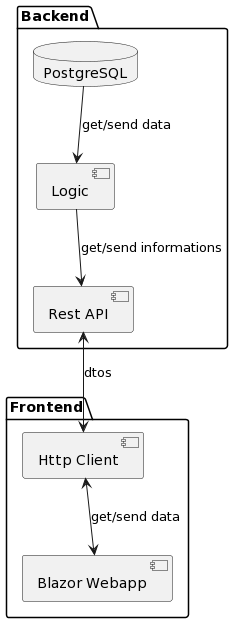
\includegraphics[scale=0.5]{pics/KomponentenDiagramm.png}
    \caption{Komponenten -- UML Diagramm}
    \label{fig:impl:KomponentenDiagramm}
\end{figure}

Die Schnittstelle zur Kommunikation auf der Seite des Frontends ist in Services pro Entität implementiert:

\begin{lstlisting}[language={[Sharp]C}, caption=Services für Kommunikation, label=lst:imp:service]
    private readonly HttpClient _http;
    public GradeService(HttpClient http)
    {
        _http = http;
    }

    public List<GradeKeyGetDto> GradeKeys { get; set; } = new List<GradeKeyGetDto>();
    public List<SchoolClassGetDto> Schooclasses { get; set;} = new List<SchoolClassGetDto>();
    public List<GradeGetDto> Grades { get; set; } = new List<GradeGetDto>();
    public List<GradeKindGetDto> Kinds { get; set; } = new List<GradeKindGetDto>();
    
    public async Task CreateGradeAsync(Grade grade)
    {
        var result = await _http.PostAsJsonAsync("/grades", grade);
        await SetGradesAsync(result);
    }
\end{lstlisting}

\newpage

Die API ist in Controllern pro Entität aufgebaut:
\begin{lstlisting}[language={[Sharp]C}, caption=API - Controller, label=lst:imp:controller]
    private readonly GradeCalculator _gradeCalculator;
    private readonly IMapper _mapper;
    private IConfiguration Config { get; }
    private ApplicationDbContext DbContext { get; }
    //private readonly ILogger<StudentsController> _logger;
    public GradeController(IConfiguration config, ApplicationDbContext dbContext, IMapper mapper, GradeCalculator gradeCalculator) 
    {
        this.Config = config;
        this.DbContext = dbContext;
        _mapper = mapper;
        _gradeCalculator = gradeCalculator;       
    }
\end{lstlisting}

\newpage
Damit der Aufbau der .NET-Solution noch klarer wird ist nun die YAML-Datei dargestellt:

\lstinputlisting[style=yaml]{input-files/docker-compose.yml}
\newpage

Die verwendeten Entitäten und ihre Relationen im Backend sind in der folgenden Abbildung dargestellt.

\begin{figure}[H]
    \centering
    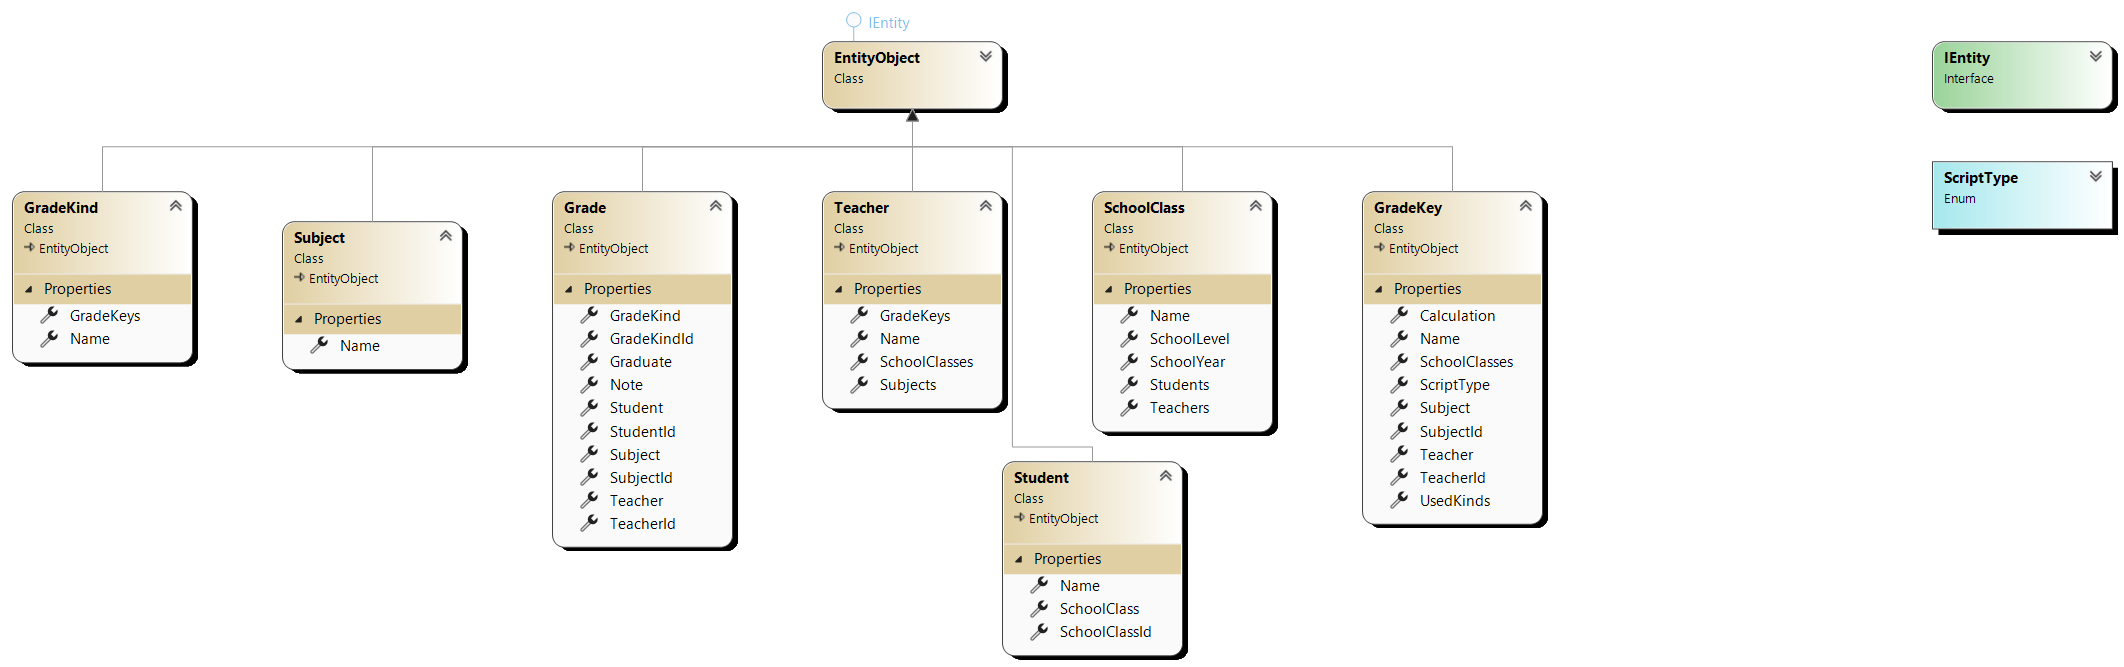
\includegraphics[scale=0.5]{pics/EntitiesClassDiagram.png}
    \caption{Entitäten -- UML Diagramm}
    \label{fig:impl:Entities}
\end{figure}




\newpage
Es gibt viele Möglichkeiten Skripte in eine Anwendung zu importieren.
Eine Möglichkeit ist die Skripte als Datei zu importieren.
Anstatt alle benötigten Daten direkt in den Code einzubetten oder sie manuell über die Befehlszeile einzugeben, 
können Entwickler*innen eine oder mehrere Dateien als Input verwenden, die das Skript dann liest und verarbeitet.

In unseren Fall werden die Datei in Blazor eingelesen.
Um das einlesen noch effizienter zu gestalten ist ein "Drag and Drop" für Dateien implementiert:

\begin{figure}[H]
    \centering
    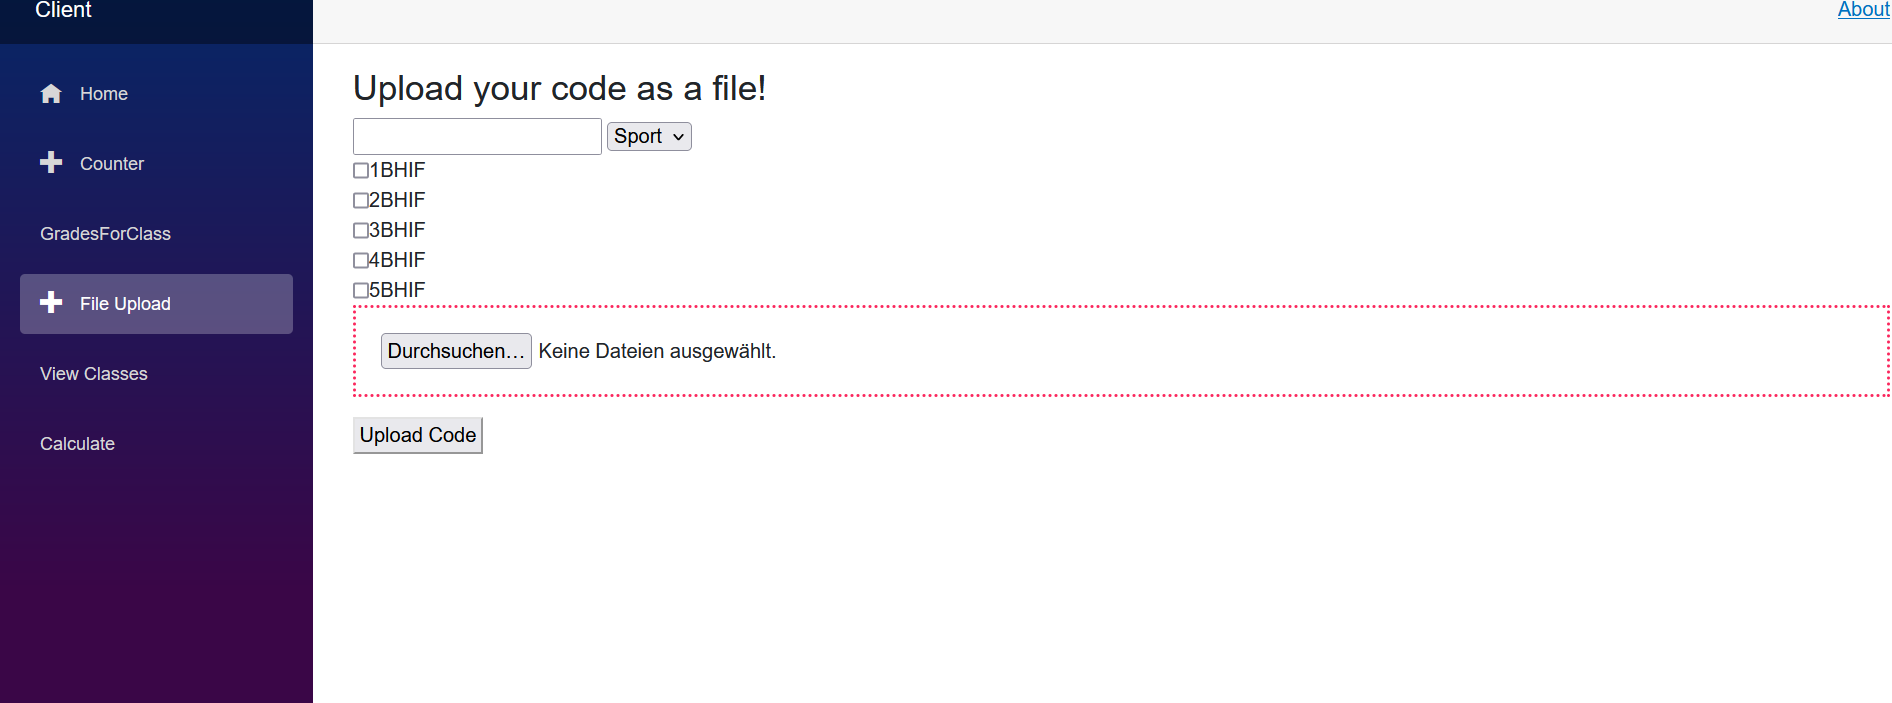
\includegraphics[scale=0.5]{pics/FileUpload.png}
    \caption{File Upload}
    \label{fig:impl:fileupload}
\end{figure}

Es folgt nun der Code:

\begin{lstlisting}[language={[Sharp]C}, caption=Code for FileUpload, label=lst:imp:fu]
    @page "/fileupload"

    @using Client.Services;
    @using global::Shared.Entities;
    @using global::Shared.Dtos;
    
    @implements IAsyncDisposable;
    @inject IJSRuntime JSRuntime;
    @inject ISubjectService SubjectService;
    @inject IGradeService GradeService;
    @inject NavigationManager NavigationManager;
    
    <h3>Upload your code as a file!</h3>
    
    <EditForm Model="@gradeKeyPost">
        <InputText id="name" @bind-Value="gradeKeyPost.Name" />
    
        <InputSelect id="subject" @bind-Value="gradeKeyPost.SubjectId">
            @foreach (var item in @SubjectService.Subjects)
            {
                <option value="@item.Id"> @item.Name </option>
            }
        </InputSelect>
    
        <CheckBoxList Data="@GradeService.Schooclasses" TextField="@((item)=>item.Name)" ValueField="@((item)=>item.Name)"
            SelectedValues="@SelectedSchoolClasses" />
    
        <div @ref="fileDropContainer" class="file-drop-zone @HoverClass" @ondragenter="OnDragEnter"
            @ondragleave="OnDragLeave" @ondragover="OnDragEnter">
            <InputFile OnChange="@OnChange" multiple />
        </div>
    
        <div class="error-message-container">
            <p>@ErrorMessage</p>
        </div>
    
        <div>
            <button type="submit" @onclick="AddGradeKeyAsync">
                Upload Code
            </button>
        </div>
        
    </EditForm>
    
    

    @code
    {
        protected List<string> SelectedSchoolClasses = new List<string>();
        private string HoverClass = string.Empty;
        void OnDragEnter(DragEventArgs e) => HoverClass = "hover";
        void OnDragLeave(DragEventArgs e) => HoverClass = string.Empty;
        IJSObjectReference? _filePasteModule = default(IJSObjectReference);
        IJSObjectReference? _filePasteFunctionReference = default(IJSObjectReference);
        ElementReference fileDropContainer;
        IBrowserFile? file;
        ScriptType scriptType;
        string stringCode = string.Empty;
        private string ErrorMessage = string.Empty;
        private const int maxAllowedFiles = 1;
        private int _userId = 1;
        private GradeKeyPostDto gradeKeyPost = new();
        protected override async Task OnInitializedAsync()
        {
            try
            {
                await SubjectService.GetSubjectsByTeacherAsync(_userId);
                await GradeService.GetSchoolclassesByTeacherAndSubjectAsync(_userId, SubjectService.Subjects.First().Id);
                await GradeService.GetAllKindsAsync();
                gradeKeyPost.SubjectId = SubjectService.Subjects.First().Id;
            }
    
            catch (Exception)
            {
                throw;
            }
        }
        private async Task AddGradeKeyAsync()
        {
            if (stringCode == string.Empty)
            {
                ErrorMessage = "Script is needed!";
            }
            var sc = GradeService.Schooclasses.SingleOrDefault(s => s.Name == SelectedSchoolClasses.First());
    
            var kinds = GradeService.Kinds.Select(k => k.Name).ToList();
            gradeKeyPost.Calculation = stringCode;
            gradeKeyPost.SchoolClasses = SelectedSchoolClasses;
            gradeKeyPost.ScriptType = scriptType;
            gradeKeyPost.UsedKinds = kinds;
            gradeKeyPost.TeacherId = _userId;
            
            await GradeService.CreateGradeKeyAsync(gradeKeyPost);
    
            //await GradeService.CalcGradesForClass(sc!.Id, _userId);
    
            NavigationManager.NavigateTo($"/calculation");
        }
    
        public async ValueTask DisposeAsync()
        {
            if (_filePasteFunctionReference != null)
            {
                await _filePasteFunctionReference.InvokeVoidAsync("dispose");
                await _filePasteFunctionReference.DisposeAsync();
            }
            if (_filePasteModule != null)
            {
                await _filePasteModule.DisposeAsync();
            }
        }
    
        protected async override Task OnAfterRenderAsync(bool firstRender)
        {
            if (firstRender)
            {
                _filePasteModule = await JSRuntime.InvokeAsync<IJSObjectReference>("import", "./js/filePaste.js");
                _filePasteFunctionReference = await _filePasteModule.InvokeAsync<IJSObjectReference>("initializeFilePaste",
                fileDropContainer, file);
            }
        }
    
        async Task OnChange(InputFileChangeEventArgs e)
        {
            stringCode = string.Empty;
            ErrorMessage = string.Empty;
    
            using var content = new MultipartFormDataContent();
    
            if (e.FileCount > maxAllowedFiles)
            {
                ErrorMessage = $"Only {maxAllowedFiles} files can be uploaded";
                return;
            }
    
    
            foreach (var file in e.GetMultipleFiles())
            {
                var isAllowed = false;
                var fileContent = new StreamContent(file.OpenReadStream());
                var info = new FileInfo(file.Name);
    
                switch (info.Extension)
                {
                    case ".lua":
                        scriptType = ScriptType.Lua;
                        isAllowed = true;
                        break;
                    case ".py":
                        scriptType = ScriptType.Python;
                        isAllowed = true;
                        break;
                    case ".csc":
                        scriptType = ScriptType.CSharpScript;
                        isAllowed = true;
                        break;
                    case ".js":
                        isAllowed = true;
                        scriptType = ScriptType.JavaScript;
                        break;
                    default:
                        ErrorMessage = "Content Type not sopported";
                        break;
                }
    
                if (isAllowed)
                {
                    stringCode = await fileContent.ReadAsStringAsync();
                }
            }
        }
    }
\end{lstlisting}
\newpage
Nach dem ein Skript hochgeladen wurde, wird man automatisch auf die Kalkulations-Seite geleitet:

\begin{figure}[H]
    \centering
    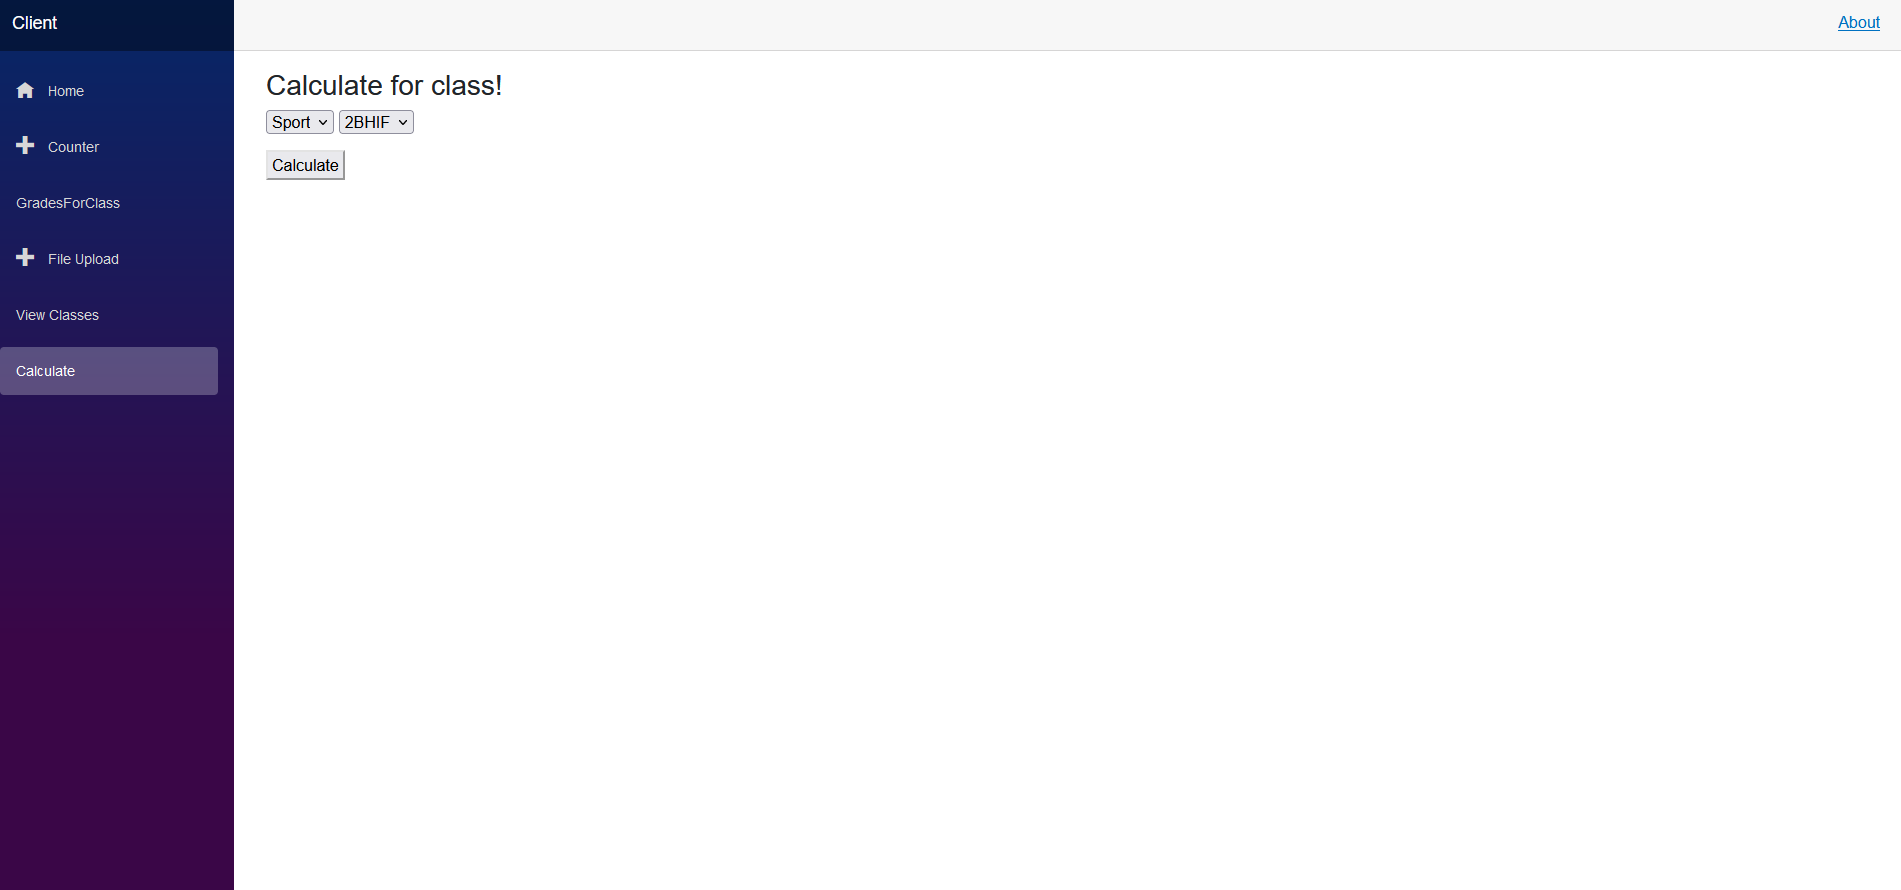
\includegraphics[scale=0.5]{pics/CalculationUI.png}
    \caption{Calculation -- UI}
    \label{fig:impl:CalculationUI}
\end{figure}

Wenn eine Berrechnung erfolgt, werden im GradeCalculator alle benötigen Daten von der Datenbank geladen und weiter zur eigentlichen Berrechnung gegeben:

\begin{figure}[H]
    \centering
    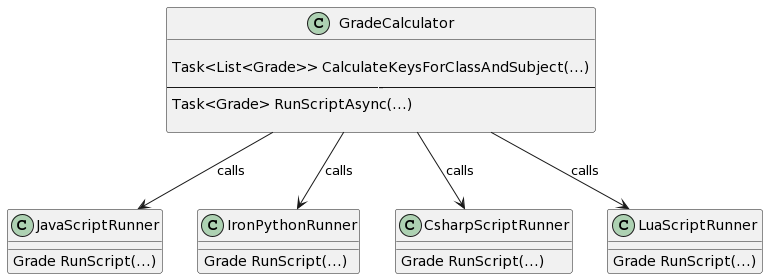
\includegraphics[scale=0.5]{pics/LogicClassDiagram.png}
    \caption{UI-- FileUpload}
    \label{fig:impl:Logic}
\end{figure}
\newpage
Es folgt nun der Code für den GradeCalculator: 

\begin{lstlisting}[language={[Sharp]C}, caption=Code for loading data for Calculation, label=lst:imp:calc]
    public async Task<List<Grade>> CalculateKeysForClassAndSubject(int schoolClassId, int subject)
    {
            var grades = await context.Grades
                .Include(g => g.Subject)
                .Include(g => g.Student)
                .Where(g => g.SubjectId == subject && g.Student!.SchoolClassId == schoolClassId)
                .ToListAsync();

            if (grades == null || grades.Count() == 0)
            {
                return new List<Grade>();
            }

            var schoolClass = await context.SchoolClasses.SingleAsync(sc => sc.Id == schoolClassId);

            var g1 = grades.First();
            var key = await context.GradeKeys
                .SingleOrDefaultAsync(k => k.SubjectId == subject && k.TeacherId == g1.TeacherId && k.SchoolClasses.Contains(schoolClass));

            if(key == null)
            {
                throw new NullReferenceException("No Key found");
            }
                
            var result = new List<Grade>();

            foreach (var item in grades.DistinctBy(g => g.StudentId).Select(g => g.StudentId))
            {
                var student = context.Students.Single(s => s.Id == item);
                var gradesForCalc =  grades.Where(g => g.StudentId == student.Id).ToList();
                // Run Script for one student
                var gradeForStudent = await this.RunScriptAsync(key, 
                                                   gradesForCalc, 
                                                   student);
                gradeForStudent.TeacherId = key.TeacherId;
                gradeForStudent.StudentId = item;
                gradeForStudent.SubjectId = key.SubjectId;
                gradeForStudent.GradeKindId = 1;
                result.Add(gradeForStudent);
            }

            return result;
        }

        
        /// Handels the script type
        private async Task<Grade> RunScriptAsync(GradeKey gradeKey, List<Grade> grades, Student student)
        {
            var result = new Grade();
            result.Student = student;
            switch (gradeKey.ScriptType)
            {
                case ScriptType.None:
                    break;
                case ScriptType.Lua:
                    result = luaScriptRunner.RunScript(gradeKey, grades);
                    break;
                case ScriptType.Python:
                    result = pythonScriptRunner.RunScript(gradeKey, grades);
                    break;
                case ScriptType.JavaScript:
                    result = jsRunner.RunScript(gradeKey, grades);
                    break;
                case ScriptType.CSharpScript:
                    result = await csScriptRunner.RunScriptAsync(gradeKey, grades);
                    break;
                default:
                    result = null;
                    break;
            }

            if (result == null)
            {
                throw new Exception("Erorr in Calculation");
            }

            result.Student = student;

            result.Note = $"{student.Name} : {DateTime.Now}";

            return result;
        }
\end{lstlisting}

\newpage
Im folgenden Abschnitt  werden einige Code-Ausschnitte betrachtet, die zeigen, wie man solche Datei-Übergaben in den untersuchten Scriptsprachen realisieren kann. 

\begin{lstlisting}[language={[Sharp]C}, caption=Code for IronPython, label=lst:imp:py]
    /// <summary>
    /// Runs Python-scripts
    /// </summary>
    public class PythonScriptRunner
    {
        private readonly ScriptEngine engine;

        public PythonScriptRunner()
        {
            this.engine = Python.CreateEngine();
        }
        public Grade RunScript(GradeKey key, List<Grade> grades)
        {
            if (key.Calculation == string.Empty || key.UsedKinds == null || grades == null)
            {
                throw new NullReferenceException("Not enough information for Calculation");
            }

            var code = key.Calculation;

            var result = new Grade();
            try
            {
                var scope = engine.CreateScope();
                engine.GetClrModule();

                var parseGrades = grades.ToArray()!;
                scope.SetVariable("grades", parseGrades);
                var source = engine.CreateScriptSourceFromString(code);
                source.Execute();
                var graduate = scope.GetVariable("graduate");
                result.Teacher = key.Teacher;
                result = Convert.ToInt32(graduate);
            }
            catch (Exception)
            {
                throw;
            }

            return result;
        }
    }
\end{lstlisting}

\newpage
Als Beispiel Skript für IronPython kann folgender Code genommen werden:
\begin{lstlisting}[language={Python},caption=IronPython-Code,label=lst:impl:ipy]
def calculate():
    makGradesCount = 0
    makGrade = 0
    testGrade = 0
    testCount = 0
    hwCount = 0
    hwGrade = 0
    
    for grade in grades:

        if grade.GradeKind.Name == 'MAK':
            makGrade = makGrade + grade.Graduate
            makGradesCount = makGradesCount + 1
        
        elif grade.GradeKind.Name == 'TEST' :
            testCount = testCount + 1
            testGrade = testGrade + grade.Graduate
        
        elif grade.GradeKind.Name == 'HOMEWORK' :
            hwCount = hwCount + 1
            hwGrade = hwGrade + grade.Graduate

    mak = makGrade / makGradesCount
    test =  testGrade / testCount
    hw = hwGrade / hwCount


    result = (mak + test + hw) / 3 

    return result


graduate = calculate()

\end{lstlisting}


\newpage

Wenn es sich um einen Javascript-Code handelt wird folgende Methode aufgerufen:

\begin{lstlisting}[language={[Sharp]C},caption=Code for Javascript,label=lst:impl:js]
    public class JavascriptRunner
    {
        public Grade RunScript(GradeKey key, List<Grade> grades)
        {
            var engine = new JintJsEngine();
            Grade result = new Grade();
            List<string>? logs = new List<string>();

            try
            {
                // Definiere eine Variable im JavaScript-Code, um die console.log-Ausgaben zu speichern
                engine.Execute("var consoleOutput = [];");

                // Definiere die console.log-Funktion im JavaScript-Code
                engine.Execute(@"
                                var console = {
                                    log: function() {
                                        consoleOutput.push(Array.from(arguments).join(' '));
                                    }
                                };
                            ");


                var gradeKindsList = JsonConvert.SerializeObject(key.UsedKinds);
                var gradesList = JsonConvert.SerializeObject(grades);

                engine.SetVariableValue("gradeKindsList", gradeKindsList);
                engine.SetVariableValue("gradesList", gradesList);

                if (key.Calculation != null)
                {
                    engine.Execute(key.Calculation);
                }

                //Die Ausgabe der console.log-Anweisungen als JSON-String
                string jsonOutput = engine.Evaluate<string>("JSON.stringify(consoleOutput)");

                // Konvertiere den JSON-String in eine Liste von strings
                if (jsonOutput != null)
                {
                    logs = JsonConvert.DeserializeObject<List<string>>(jsonOutput);

                    if (logs != null)
                    {
                        DisplayOutput(logs);   
                    }
                }

                // Get Return from Script
                var resultGrade = engine.GetVariableValue("result");

                result.Teacher = key.Teacher;
                result.Graduate = Convert.ToInt32(resultGrade);
            }
            catch (Exception)
            {
                result.Teacher = null;
                result.Graduate = 0;
            }
            return result;
        }

        private static void DisplayOutput(List<string> logs)
        {
            foreach (string output in logs)
            {
                Debug.WriteLine(output);
            }
        }
    }
\end{lstlisting}
\newpage
Als Beispiel hierfür ein Skript:
\begin{lstlisting}[language={JavaScript},caption=Javascript-Skript,label=lst:impl:jstest]
var grades = JSON.parse(gradesList);
var gradeKinds = JSON.parse(gradeKindsList);

function calculate() {
    let makCounter = 0;
    let testCounter = 0;
    let homeworkCounter = 0;

    let mak = 0;
    let test = 0;
    let homework = 0;

    for (let i = 0; i < grades.length; i++) {

        if (grades[i].GradeKind.Name == 'MAK') {
            mak += grades[i].Graduate;
            makCounter++;
        }
        if (grades[i].GradeKind.Name == 'TEST') {
            test += grades[i].Graduate;
            testCounter++;
        }
        if (grades[i].GradeKind.Name == 'HOMEWORK') {
            homework += grades[i].Graduate;
            homeworkCounter++;
        }
    }
    return ((mak / makCounter) + (test / testCounter) + (homework / homeworkCounter)) / 3;
}
var result = calculate();
console.log('Wert: ' +grades[1].GradeKind.Name);
\end{lstlisting}


\newpage
Bei einem Lua-Skript wird folgende Methode aufgerufen:

\begin{lstlisting}[language={[Sharp]C},caption=Code for NLua,label=lst:impl:nlua]
    /// <summary>
    /// Runs lua-scripts
    /// </summary>
    public class LuaScriptRunner
    {
        private readonly Lua state;

        public LuaScriptRunner()
        {
            this.state = new Lua();
        }

        public Grade RunScript(GradeKey key, List<Grade> grades)
        {
            if (key.Calculation == string.Empty || key.UsedKinds == null || grades == null)
            {
                throw new NullReferenceException("Not enough information for Calculation");
            }

            var code = key.Calculation;

            var result = new Grade();
            try
            {
                state.DoString(code);
                state.LoadCLRPackage();
                state["grades"] = grades;
                state.DoString(@"graduate = calculate()");
                result.Teacher = key.Teacher;
                var gr = state["graduate"];
                if (gr != null) 
                {
                    result.Graduate = Convert.ToInt32(gr);
                }
            }
            catch (Exception)
            {
                throw;
            }

            return result;
        }
    }
\end{lstlisting}
\newpage
Hierfür kann folgendes Skript verwendet werden:
\begin{lstlisting}[language={[5.0]Lua},caption=Lua Example,label=lst:impl:luascript]
function calculate()

    local makGradesCount = 0
    local makGrade = 0
    local testGrade = 0
    local testCount = 0
    local hwCount = 0
    local hwGrade = 0

    for countGrade = 0, grades.Count - 1 do 
        if grades[countGrade].GradeKind.Name == 'MAK' then
            makGrade = makGrade + grades[countGrade].Graduate
            makGradesCount = makGradesCount + 1
        elseif grades[countGrade].GradeKind.Name == 'TEST' then
            testCount = testCount + 1
            testGrade = testGrade + grades[countGrade].Graduate
        elseif grades[countGrade].GradeKind.Name == 'HOMEWORK' then
            hwCount = hwCount + 1
            hwGrade = hwGrade + grades[countGrade].Graduate
        end
    end

    local result = ((makGrade / makGradesCount) + ( testGrade / testCount ) + (hwGrade / hwCount)) / 3     

    return math.floor(result)
end
\end{lstlisting}
\newpage

Für ein Csharpscript wird folgender Code ausgeführt:

\begin{lstlisting}[language={[Sharp]C},caption=Code for CsharpScripting,label=lst:impl:csc]
    public class CsScriptMicrosoftRunner
    {
        public async Task<Grade> RunScriptAsync(GradeKey key, List<Grade> grades)
        {
            var result = new Grade();
            var globals = new Globals { GradeKey = key, Grades = grades };
            var options = ScriptOptions.Default
                .WithEmitDebugInformation(true);

            try
            {
                var state = await CSharpScript.RunAsync(key.Calculation, options, globals: globals);
                WriteAllVariablesFromScript(state.Variables);

                double resultGrade = 0.0;
                foreach (var variable in state.Variables)
                {
                    if (variable.Name == "result")
                    {
                        resultGrade = (double)variable.Value;
                    }
                }

                result.Teacher = key.Teacher;
                result.Graduate = Convert.ToInt32(resultGrade);

            }
            catch (Exception)
            {
                result.Teacher = null;
                result.Graduate = 0;
            }

            return result;
        }

        private static void WriteAllVariablesFromScript(ImmutableArray<ScriptVariable> variables)
        {
            foreach (var variable in variables)
            {
                Debug.WriteLine(variable.Name + ": " + variable.Value);
            }
        }

        public class Globals
        {
            public GradeKey? GradeKey;
            public List<Grade>? Grades;
        }
    }
\end{lstlisting}

\newpage

Für ein Csharpscript wird folgender Code ausgeführt:
    
\begin{lstlisting}[language={[Sharp]C},caption=Csharpscript,label=lst:impl:csctest]
    int makCounter = 0;
int testCounter = 0;
int homeworkCounter = 0;

int mak = 0;
int test = 0;
int homework = 0;

foreach (var item in Grades)
{
    if (item.GradeKind.Name == "MAK")
    {
        mak += item.Graduate;
        makCounter++;
    }
    if (item.GradeKind.Name == "TEST")
    {
        test += item.Graduate;
        testCounter++;
    }
    if (item.GradeKind.Name == "HOMEWORK")
    {
        homework += item.Graduate;
        homeworkCounter++;
    }
}

double result = ((mak / makCounter) + (test / testCounter) + (homework / homeworkCounter)) / 3.0;
\end{lstlisting}

Nach der Berrechnung werden die Jahresnoten in einer Tabelle dargestellt:

\begin{figure}[H]
    \centering
    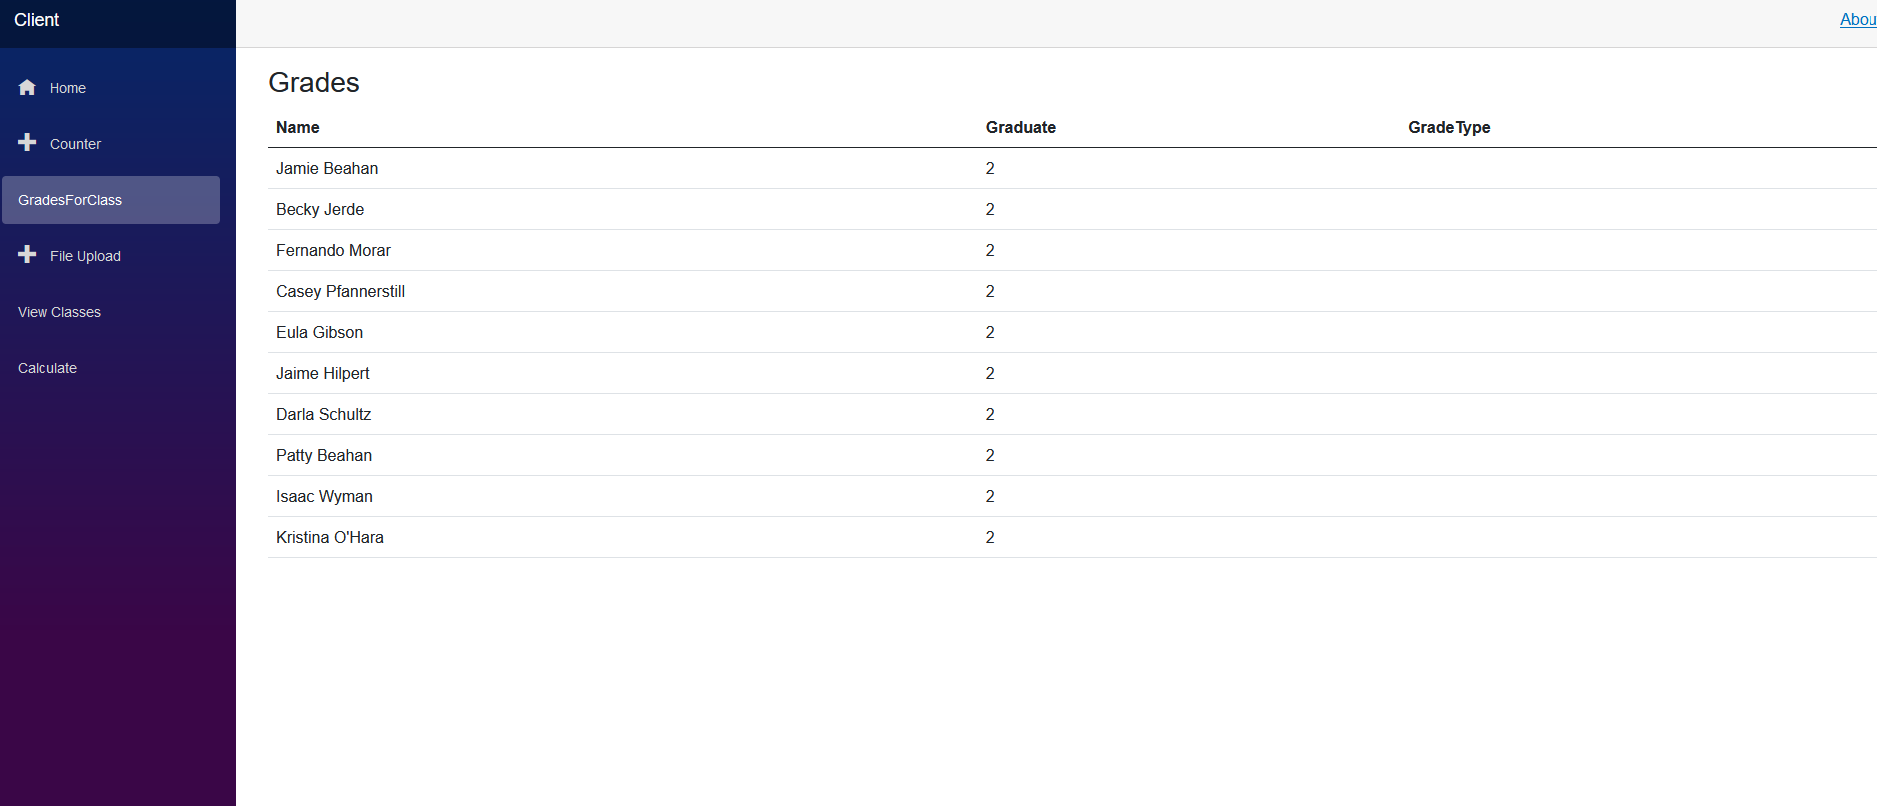
\includegraphics[scale=0.5]{pics/GradesForClass.png}
    \caption{UI -- Jahesnoten}
    \label{fig:impl:GradesForClass}
\end{figure}



\newpage
\section{Unit-Tests zur Überprüfung der Notenberechnung}
\setauthor{Philipp Füreder}

Eine der zentralen Komponenten unserer Beispielanwendung war die Implementierung von 
Skripten zur Notenberechnung in .NET-Anwendungen zur Laufzeit. Um die Zuverlässigkeit und 
Genauigkeit dieser Skripte sicherzustellen, haben wir einen Satz von Unit-Tests entwickelt 
und durchgeführt. Dieser Ansatz gewährleistet nicht nur die Integrität des Codes, 
sondern bietet auch eine robuste Basis für zukünftige Erweiterungen und Anpassungen.

\subsection*{Auswahl der Testfälle}
Die Testfälle wurden so ausgewählt, um ein breites Spektrum an Szenarien abzudecken, 
die in realen Anwendungen vorkommen könnten. Dazu gehören Standardfälle, Grenzfälle und 
auch potenzielle Fehlerzustände. Das hat uns ermöglicht, die Robustheit für unsere Test-Scripts 
umfassend zu überprüfen.

\subsection*{Ergebnisse der Unit-Tests}
Alle entwickelten Skripte zur Notenberechnung haben die Tests letztenendes erfolgreich bestanden. 
Dies gab uns ein hohes Maß an Vertrauen in die Funktionsfähigkeit und Zuverlässigkeit der 
implementierten Lösungen. Darüber hinaus haben die Tests dazu beigetragen, einige nicht 
offensichtliche Fehler und Unklarheiten im ursprünglichen Design zu identifizieren, 
die wir entsprechend beheben konnten.

\newpage
\subsection*{Testbeispiel}

In folgendem Testbeispiel haben wir ein C\#-Skript getestet:

\begin{lstlisting}[language={[Sharp]C},caption=Test for CsharpScripting,label=lst:impl:csc]
[TestMethod]
    public void CsScript_T02()
    {
        List<Grade> grades = new List<Grade>
        {
            new Grade { GradeKind = gradeKinds.Single(g => g.Name =="MAK") , Graduate = 1 },
            new Grade { GradeKind = gradeKinds.Single(g => g.Name =="MAK") , Graduate = 1 },
            new Grade { GradeKind = gradeKinds.Single(g => g.Name =="MAK") , Graduate = 1 },
            new Grade { GradeKind = gradeKinds.Single(g => g.Name =="MAK") , Graduate = 2 },
            new Grade { GradeKind = gradeKinds.Single(g => g.Name =="MAK") , Graduate = 1 },
            new Grade { GradeKind = gradeKinds.Single(g => g.Name == "TEST"), Graduate = 1},
            new Grade { GradeKind = gradeKinds.Single(g => g.Name == "TEST"), Graduate = 2},
            new Grade { GradeKind = gradeKinds.Single(g => g.Name == "TEST"), Graduate = 3},
            new Grade { GradeKind = gradeKinds.Single(g => g.Name == "TEST"), Graduate = 4},
            new Grade { GradeKind = gradeKinds.Single(g => g.Name == "TEST"), Graduate = 2},
            new Grade { GradeKind = gradeKinds.Single(g => g.Name == "HOMEWORK"), Graduate = 1},
            new Grade { GradeKind = gradeKinds.Single(g => g.Name == "HOMEWORK"), Graduate = 2},
            new Grade { GradeKind = gradeKinds.Single(g => g.Name == "HOMEWORK"), Graduate = 3},
            new Grade { GradeKind = gradeKinds.Single(g => g.Name == "HOMEWORK"), Graduate = 4},
            new Grade { GradeKind = gradeKinds.Single(g => g.Name == "HOMEWORK"), Graduate = 5},

        };

        var code = File.ReadAllText("test.cs");
        var key = new GradeKey { Name = "CsScriptTest", UsedKinds = gradeKinds, Calculation = code };

        var result = CsScriptRunner.RunScript(key, grades);

        Assert.AreEqual(2, result.Graduate, "Calculation is right");
\end{lstlisting}

Dabei beinhaltet die Liste "grades" Schulnoten von drei verschiedenen Typen:
\begin{itemize}
    \item MAK (Mitarbeitskontrolle)
    \item Test
    \item Homework
\end{itemize}


\newpage
\subsection*{Test-Skript}
Dieses Test-Skript haben wir geschrieben um die Funktionalitäten und Notenberechnungen zu testen.
Einfachheitshalber wird in diesem Skript jeder Notentyp äquivalent gerechnet.

\begin{lstlisting}[language={[Sharp]C},caption=CsharpScript-Testscript,label=lst:impl:csc]
int makCounter = 0;
int testCounter = 0;
int homeworkCounter = 0;

int mak = 0;
int test = 0;
int homework = 0;

foreach (var item in Grades)
{
    if (item.GradeKind.Name == "MAK")
    {
        mak += item.Graduate;
        makCounter++;
    }
    if (item.GradeKind.Name == "TEST")
    {
        test += item.Graduate;
        testCounter++;
    }
    if (item.GradeKind.Name == "HOMEWORK")
    {
        homework += item.Graduate;
        homeworkCounter++;
    }
}

return ((mak / makCounter) + (test / testCounter) + (homework / homeworkCounter)) / 3.0;
\end{lstlisting}

Das Skript unterscheidet zwar zwischen allen Notentypen, wertet jedoch alle gleich 
und berechnet den Durchschnitt.
